\documentclass[aspectratio=169,11pt]{beamer}
\usepackage[utf8]{inputenc}
\usepackage[T1]{fontenc}
\usepackage{lmodern,amsmath,amssymb,booktabs,graphicx,listings}
\definecolor{ink}{HTML}{173342}
\definecolor{teal}{HTML}{126D87}
\definecolor{rust}{HTML}{C96A24}
\setbeamercolor{normal text}{fg=ink,bg=white}
\setbeamercolor{structure}{fg=teal}
\setbeamercolor{frametitle}{fg=ink}
\setbeamercolor{block title}{fg=white,bg=teal}
\setbeamercolor{block body}{fg=ink,bg=teal!6}
\setbeamertemplate{navigation symbols}{}
\setbeamertemplate{footline}{\hfill\usebeamercolor[fg]{structure}\scriptsize Ide \& Talam\`as (2025)\quad\insertframenumber/\inserttotalframenumber\hspace{5mm}\vspace{3mm}}
\setbeamertemplate{itemize item}{\small\raise1pt\hbox{$\bullet$}}
\setbeamersize{text margin left=9mm,text margin right=9mm}
\setbeamerfont{frametitle}{size=\Large,series=\bfseries}
\setbeamerfont{title}{size=\LARGE,series=\bfseries}
\setlength{\parskip}{5pt}
\newcommand{\ai}{a}
\newcommand{\wa}{w^{*}}
\newcommand{\wc}{w^{\star}}
\newcommand{\src}[1]{\vfill{\scriptsize\color{gray}Source: arXiv v11, #1.}}
\lstset{basicstyle=\ttfamily\scriptsize,columns=fullflexible,breaklines=true,showstringspaces=false,frame=single,rulecolor=\color{teal!35},backgroundcolor=\color{teal!3},aboveskip=4pt,belowskip=4pt,escapeinside={(*@}{@*)}}
\title{Artificial Intelligence in the Knowledge Economy}
\subtitle{Capability, autonomy, and the price of expertise}
\author{davidolano03}
\institute{Ide \& Talam\`as (2025), Journal of Political Economy\\[5pt]
\href{https://github.com/davidolano03/ai-05-ide}{\texttt{github.com/davidolano03/ai-05-ide}}}
\date{Course Repository 5}
\begin{document}

\begin{frame}
\titlepage
\vspace{-7mm}
\centering\footnotesize Source read: arXiv v11, title page dated February 25, 2025 (35 pages)
\end{frame}

\begin{frame}{The economic question}
Knowledge can be copied into AI agents. Human time cannot.
\begin{columns}[T]
\column{.48\textwidth}
\begin{block}{Capability: what does AI know?}
An agent with knowledge $\ai$ solves a fraction $\ai$ of problems.
\end{block}
\column{.48\textwidth}
\begin{block}{Autonomy: what may AI do?}
Autonomous AI can produce and advise. A co-pilot can only advise.
\end{block}
\end{columns}
\medskip
Who gains at the bottom, who gains at the top, and how much does the economy produce?

The comparison is between equilibria: occupations, matches, and wages all adjust.
\src{Sections 3 and 6}
\end{frame}

\begin{frame}{A firm allocates scarce problem-solving time}
One worker has knowledge $z$ and encounters $x\sim U[0,1]$. A solver knows $s>z$.
\[
\underbrace{n(z)}_{\text{workers}}\,
\underbrace{(1-z)}_{\text{questions per worker}}\,
\underbrace{h}_{\text{time per question}}=1
\quad\Longrightarrow\quad n(z)=\frac{1}{h(1-z)}.
\]
\[
\Pi=n(z)\,[s-w(z)]-w(s).
\]
People maximize income. Firms choose their structure and hires; competition gives zero profits and market clearing.

More worker knowledge saves solver time. More solver knowledge helps every worker in the team.
\src{pp. 10--13. Each question costs time even if the solver cannot answer}
\end{frame}

\begin{frame}{Conditions behind the main results}
\small
\begin{itemize}
\item Unit mass of humans, $z\in[0,1]$, with continuous, strictly positive density $g$.
\item Exogenous, observable knowledge; one unit of time per person; risk neutrality.
\item Competitive firms, no fixed costs, at most two layers, abundant opportunities.
\item $0<h<h_0(G)<1$: no independent human producers before AI.
\item One AI capability $\ai\in[0,1)$, common access, one agent per unit of compute.
\item Compute is abundant relative to human time. A sufficient condition is
\[
\mu>\int_0^{\ai}h(1-z)\,dG(z)+\frac{1-G(\ai)}{h(1-\ai)}.
\]
\item Autonomy comparisons hold $G,h,\ai,\mu$ fixed and retain the two-layer limit.
\end{itemize}
\src{pp. 9--14, 18 and 26. In particular, $\ai=1$ is excluded}
\end{frame}

\begin{frame}{Proposition 5: bottom gains require enough capability}
Write $w$ for pre-AI wages and $\wa$ for autonomous-AI wages. Define
\[
B=\{z\in[0,\ai]:\wa(z)>w(z)\},\qquad
T=\{z\in[\ai,1]:\wa(z)>w(z)\}.
\]
\begin{block}{Under the baseline conditions}
\[
B\ne\varnothing\quad\Longleftrightarrow\quad \ai>\bar a,
\qquad \bar a\in\operatorname{int}W.
\]
\[
T\ne\varnothing\qquad\text{for every }\ai\in[0,1).
\]
\end{block}
Here $W$ is the set of workers \emph{before} AI. Winners occupy tails of the distribution; the human type $z=\ai$ loses.
\src{pp. 24--25. Top gains depend on $h<h_0$ and $\ai<1$}
\end{frame}

\begin{frame}{Proposition 6: the co-pilot threshold is $w(0)$}
Let $\wc$ denote wages with non-autonomous AI.
\begin{columns}[T]
\column{.47\textwidth}
\begin{block}{$\ai\le w(0)$}
No AI adoption in equilibrium. Human occupations and wages stay at their pre-AI values.
\end{block}
\column{.49\textwidth}
\begin{block}{$\ai>w(0)$}
The least knowledgeable use AI. Some people strictly gain, and some strictly lose.
\end{block}
\end{columns}
\medskip
The equilibrium is unique and efficient. It maximizes labor income among feasible co-pilot allocations.
\[
r^\star=0\qquad\text{because some compute is idle.}
\]
The pre-AI wage $w(0)$ includes the value of organizational support. A co-pilot must beat that outside option.
\src{pp. 26--27; AI users lie below human-assisted workers, independent producers, and solvers}
\end{frame}

\begin{frame}{Proposition 6: comparisons and strictness}
\small
Under the same baseline conditions:
\begin{align*}
Y^*&>Y^\star,\\
\exists z\in(0,1]:\quad \wc(z)&\le w(z),\\
\exists\varepsilon_b>0\ \forall z\in[0,\varepsilon_b):\quad
\wc(z)&\ge\max\{w(z),\wa(z)\},\\
\exists\varepsilon_t>0\ \forall z\in(1-\varepsilon_t,1]:\quad
\wc(z)&\le\wa(z).
\end{align*}
The second and third inequalities are strict if $\ai>w(0)$.
The last is strict for $z\ne1$; the endpoint only has a weak claim.

These are local tail comparisons, not rankings for every worker.
\src{Proposition 6, p. 27. $Y$ means total output, not labor income}
\end{frame}

\begin{frame}{Why autonomy changes the opportunity cost of advice}
\begin{columns}[T]
\column{.48\textwidth}
\begin{block}{Autonomous AI}
Spare compute can produce, so $r^*=\ai$.
\[
\wa(z)=\ai-h(1-z)\ai
\]
for a human worker using AI advice.
\[
\wa(s)=\frac{s-\ai}{h(1-\ai)}
\]
for a human solver supervising AI.
\end{block}
\column{.48\textwidth}
\begin{block}{Non-autonomous AI}
Spare compute is idle, so $r^\star=0$.
\[
\wc(z)=\ai
\]
for a human worker using AI advice.

AI cannot supply routine workers to human experts. It can compete with experts as a solver.
\end{block}
\end{columns}
\src{pp. 19--20 and 26--27. These formulas apply to the stated active occupations}
\end{frame}

\begin{frame}{A three-type economy we can solve by hand}
\[
(z_L,z_M,z_H)=(0,\tfrac12,1),\quad
(m_L,m_M,m_H)=(\tfrac12,\tfrac3{10},\tfrac15),\quad h=\tfrac12.
\]
\small
Let $x_{ij}$ measure workers of type $i$ assisted by type $j$.
An allocation $(x_{LM},x_{LH},x_{MH})=(\tfrac15,\tfrac3{10},\tfrac15)$ uses all resources.
\[
w_L+\tfrac12 w_M=\tfrac12,\quad
w_L+\tfrac12 w_H=1,\quad
w_M+\tfrac14 w_H=1.
\]
\[
\boxed{(w_L,w_M,w_H)=(\tfrac15,\tfrac35,\tfrac85)},\qquad Y=\tfrac35.
\]
Wages exceed independent output, so unused single-person firms cannot profit.
\vfill\footnotesize Own finite model: divisible masses, three knowledge atoms. This changes the paper's domain.
\end{frame}

\begin{frame}{The capability threshold comes from one subtraction}
\small
Autonomous AI, $\mu=10$, $0\le\ai\le1/3$. Low types work with middle types; remaining middle and high types supervise AI.
\[
\wa_H=2,\qquad \wa_M=\frac{1-2\ai}{1-\ai},\qquad
\wa_L=\frac12-\frac12\wa_M=\frac{\ai}{2(1-\ai)}.
\]
\begin{block}{The sign of the gain}
\[
\wa_L-\frac15=\frac{7\ai-2}{10(1-\ai)}
\quad\Longrightarrow\quad
\wa_L>\frac15\ \Longleftrightarrow\ \ai>\frac27.
\]
\end{block}
At $\ai=2/7$ there is equality. At $\ai=1/10$ the low wage falls to $1/18$; at $\ai=3/10$ it rises to $3/14$.

Autonomy is unchanged. Capability changes the sign.
\end{frame}

\begin{frame}{Same people, different AI roles}
\centering
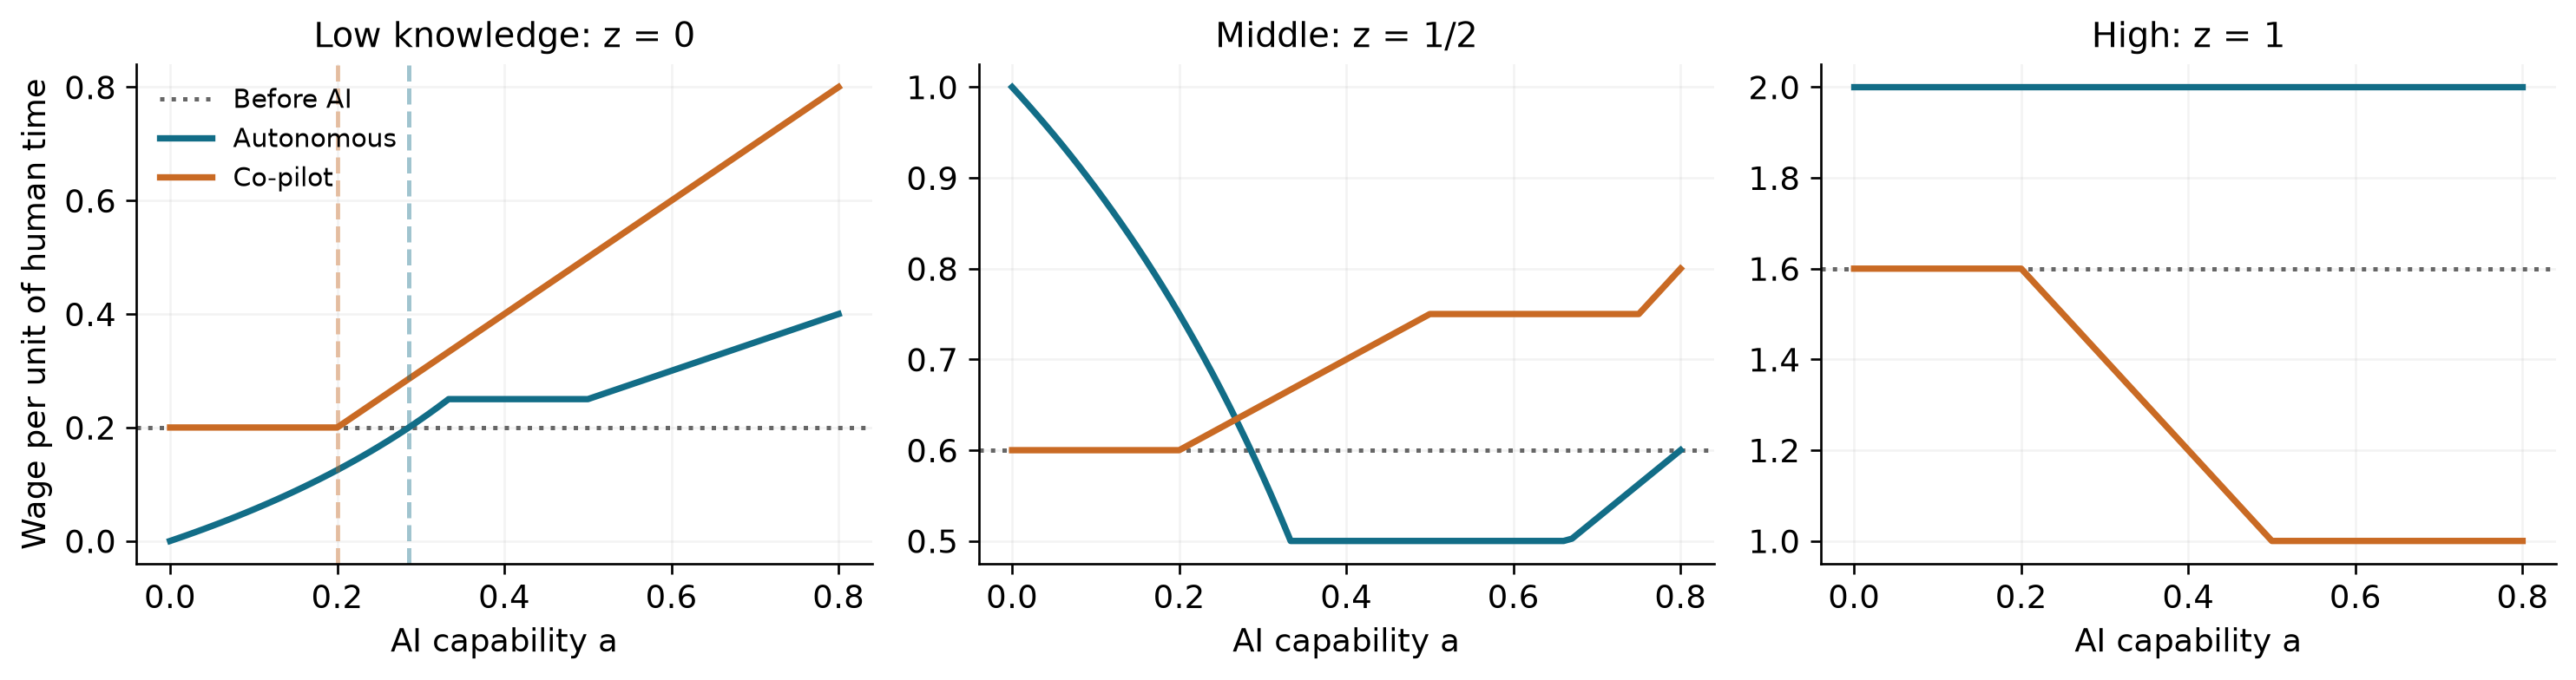
\includegraphics[width=\textwidth]{figures/wages.png}
\small
Own three-type model, $h=1/2$, $\mu=10$. Dotted lines: wages before AI.

The low-type thresholds are $1/5$ for co-pilots and $2/7$ for autonomy.
Low types can gain from autonomy while still using human supervisors.
\end{frame}

\begin{frame}{More output does not mean everyone earns more}
\centering
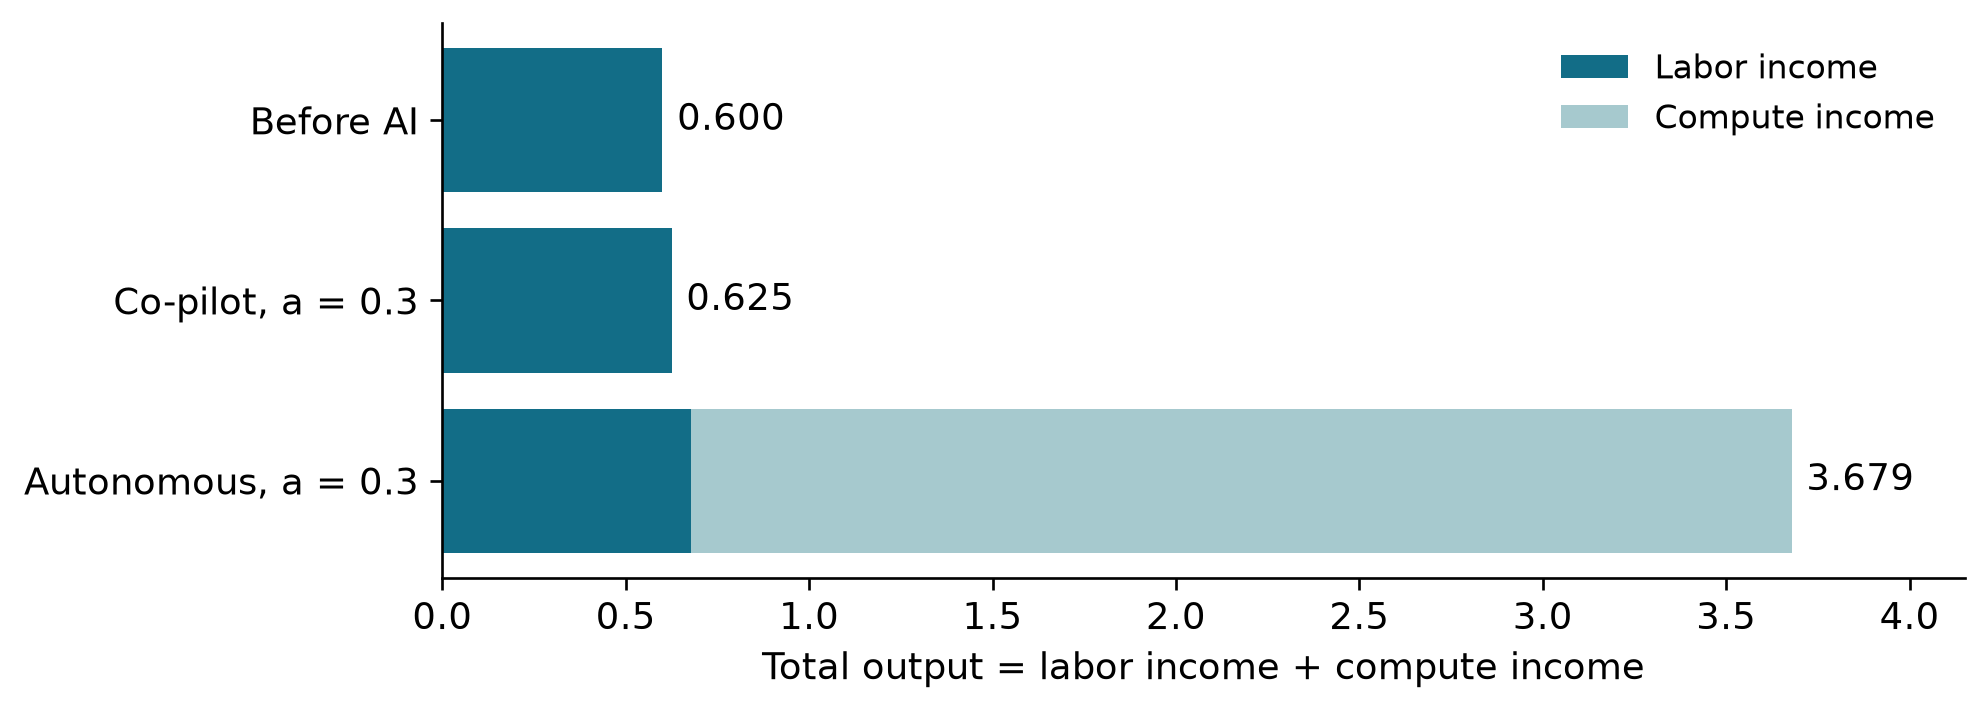
\includegraphics[width=.89\textwidth]{figures/output.png}
\par\medskip
\small
At $\ai=0.3$, autonomous labor income is $19/28\approx0.679$; total output is $103/28\approx3.679$.

The difference includes $\mu r=3$ of compute income. Co-pilot output equals labor income because its compute rent is zero.
\end{frame}

\begin{frame}{What the computation checks}
\[
\max_{x\ge0}\ c^\top x\quad\text{s.t. }Ax\le b
\qquad\longleftrightarrow\qquad
\min_{p\ge0}\ b^\top p\quad\text{s.t. }A^\top p\ge c.
\]
Columns are feasible firm activities. Resources are human types and compute. Dual prices are wages and the compute rent.
\begin{itemize}
\item Exact symbolic check of the hand algebra with SymPy.
\item 166 equilibria: feasibility, zero duality gap, and complementarity at $10^{-8}$ tolerance.
\item Wage ranges on the optimal dual face detect non-unique prices.
\end{itemize}
\small
A two-type control admits multiple wages. Another violates top gains after changing the paper's domain. Neither is a refutation of its continuum theorem.
\end{frame}

% Archivo provisional. Se reemplaza con evidencia de la corrida propia al terminar.
\begin{frame}{Lean: formalization in progress}
\[
0\le a\le\tfrac13\quad\Longrightarrow\quad
\left(\frac{a}{2(1-a)}>\frac15\ \Longleftrightarrow\ a>\frac27\right).
\]
\begin{block}{Run status}
Own AppliedModelingLib run with GPT-5.6 Sol and \texttt{xhigh}. Source pinned to arXiv v11.
\end{block}
The final slide will identify a checked declaration and proof fragment, its assumptions and its relation to the paper.

No successful Lean build or source-equivalence claim is asserted in this provisional slide.
\end{frame}


\begin{frame}{Handwritten check: time and resource constraints}
\begin{columns}[T]
\column{.54\textwidth}\centering
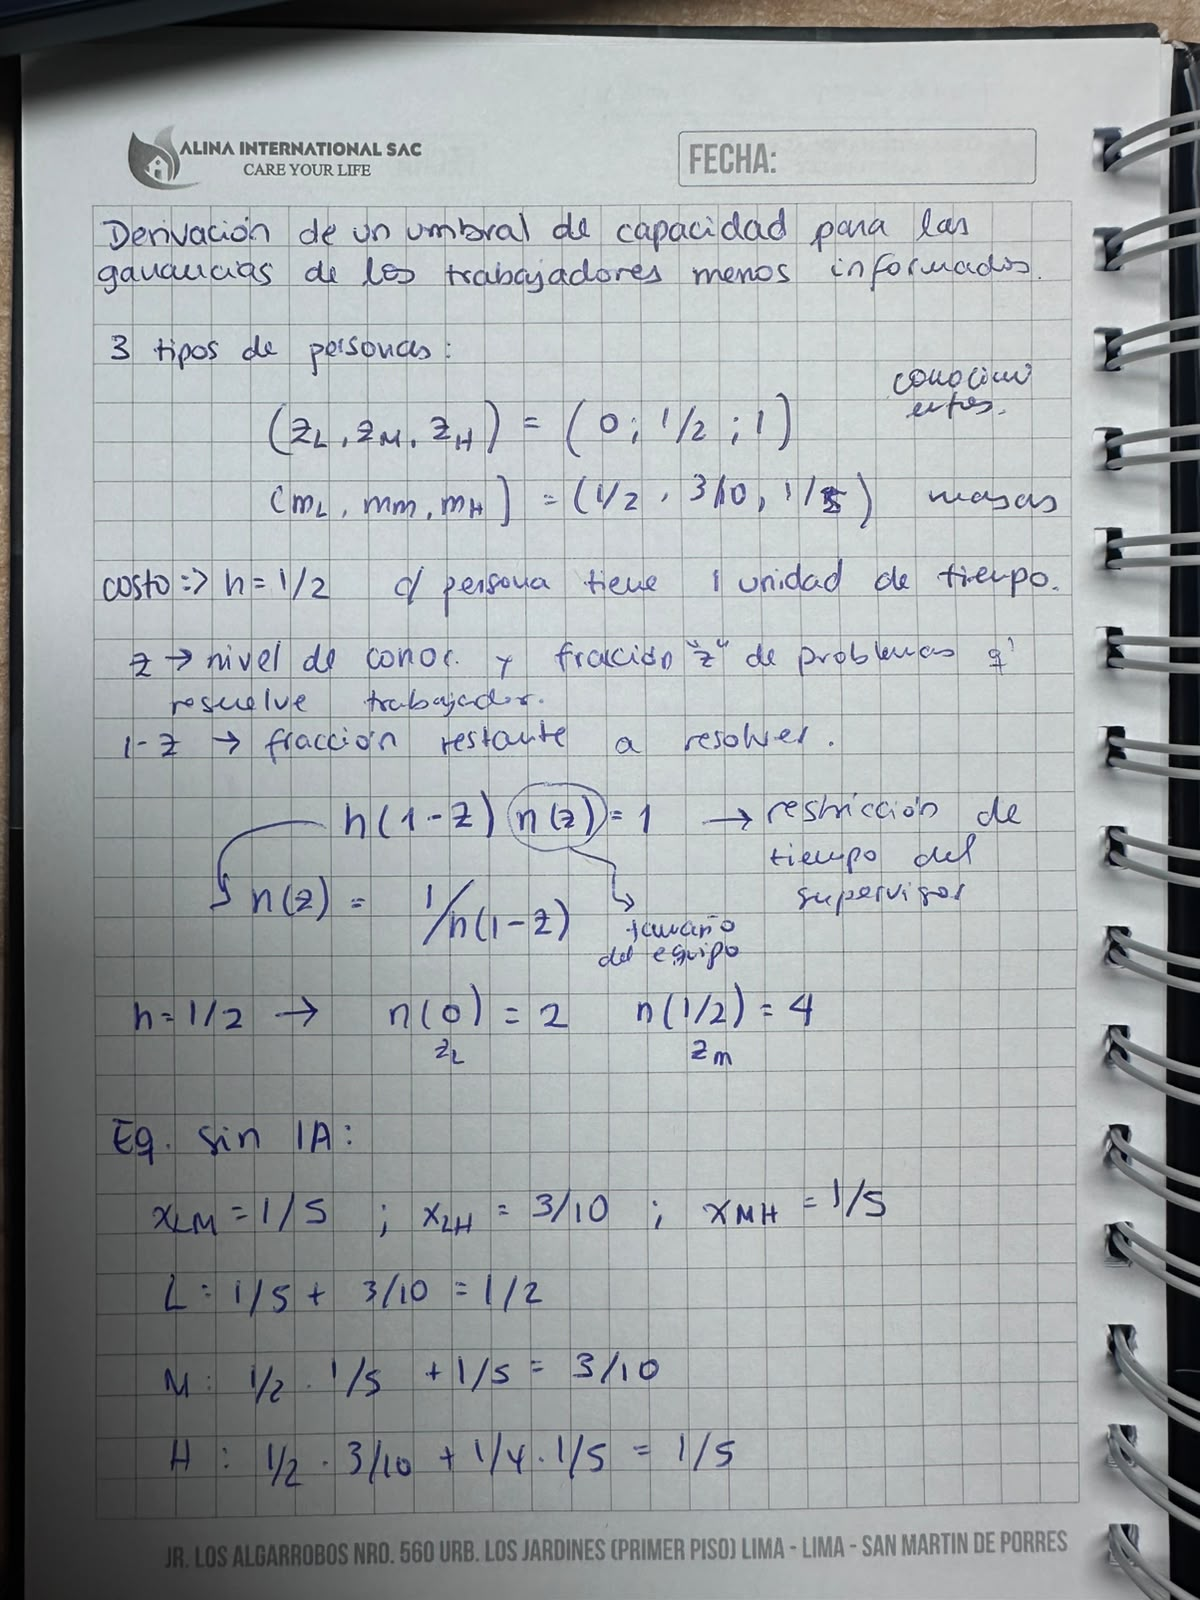
\includegraphics[trim={75bp 70bp 100bp 780bp},clip,width=\linewidth,height=.73\textheight,keepaspectratio]{hand/derivacion-01.jpeg}
\column{.43\textwidth}\small
The handwritten calculation checks solver time:
\[
h(1-z)n(z)=1.
\]
For $h=1/2$, a solver can assist two low-type workers or four middle-type workers.

The proposed allocation uses every type's available time. Zero profit then gives
\[
(w_L,w_M,w_H)=\left(\tfrac15,\tfrac35,\tfrac85\right).
\]
\footnotesize Original student photographs appear in full in the appendix.
\end{columns}
\end{frame}

\begin{frame}{Handwritten check: the threshold and the verdict}
\small
Autonomous AI, $\mu=10$, $0\le a\le1/3$. The handwritten comparison is
\[
\wa_L=\frac{a}{2(1-a)}>\frac15
\quad\Longleftrightarrow\quad 7a>2
\quad\Longleftrightarrow\quad a>\frac27.
\]
\begin{columns}[c]
\column{.61\textwidth}\centering
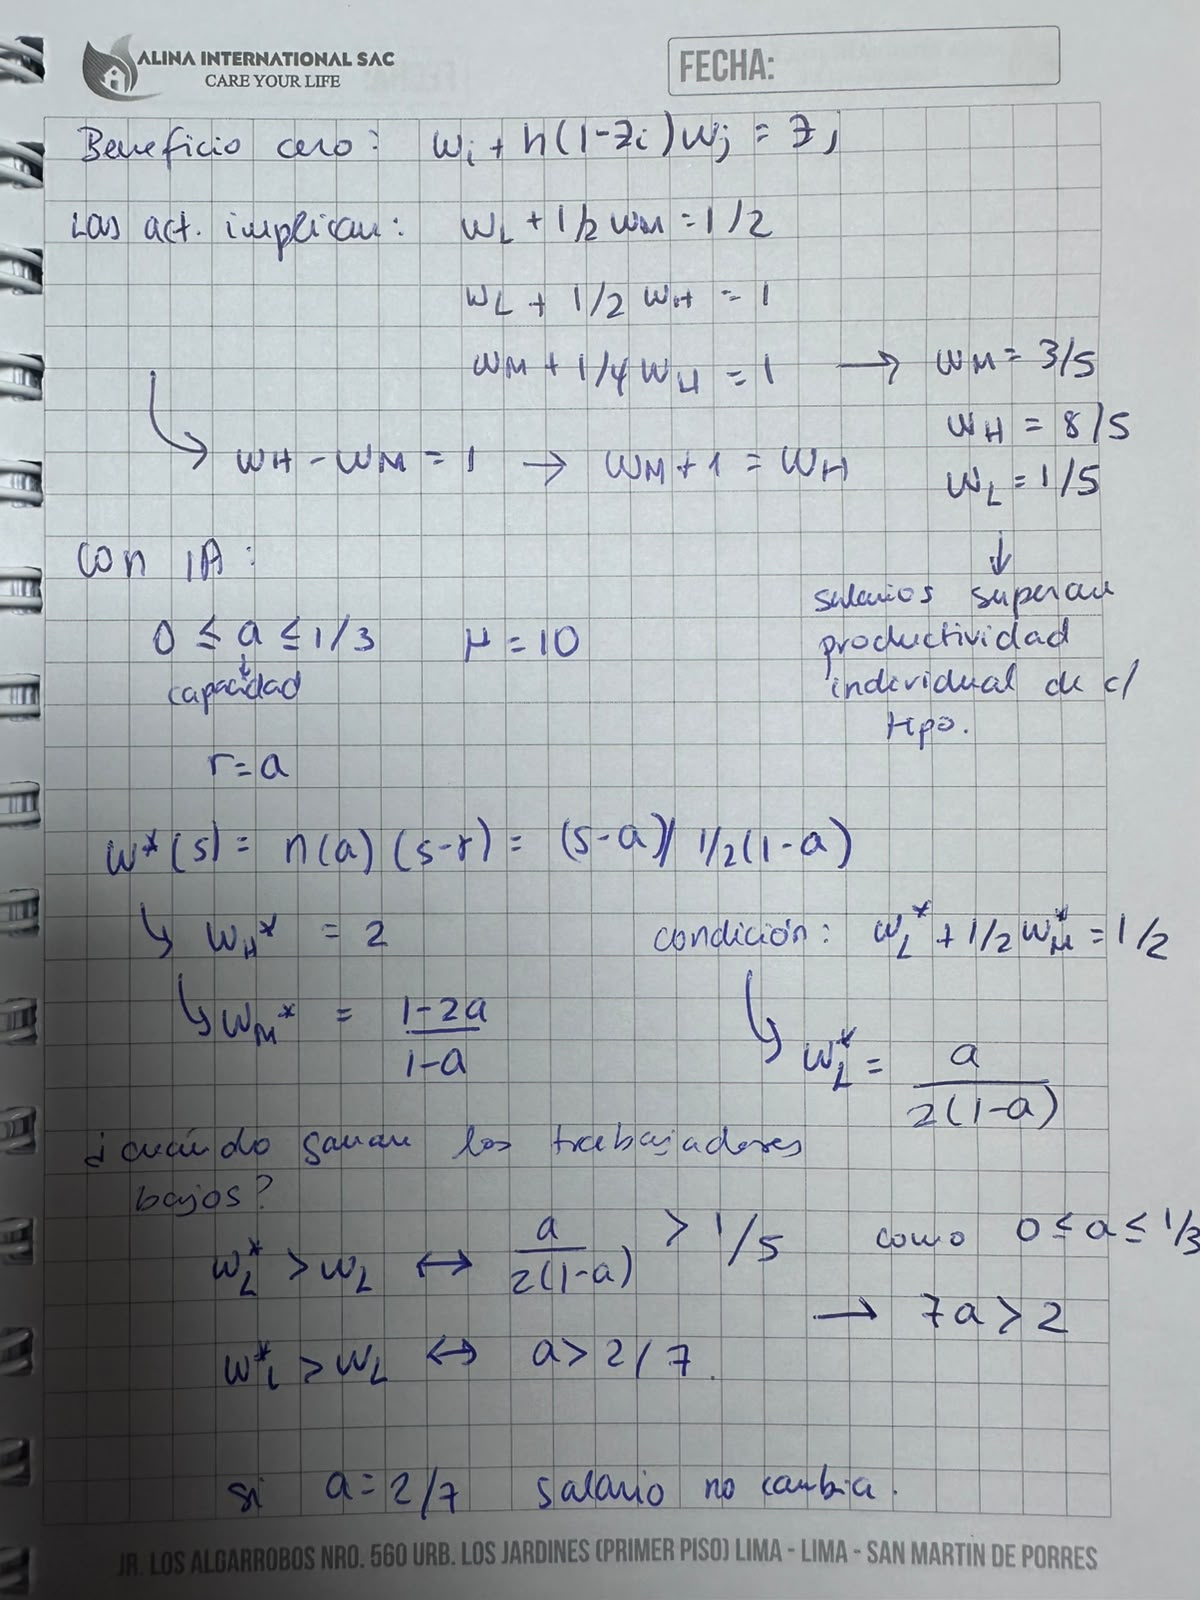
\includegraphics[trim={50bp 70bp 45bp 1110bp},clip,width=\linewidth]{hand/derivacion-02.jpeg}
\column{.36\textwidth}\small
Since $2(1-a)>0$, multiplication preserves the inequality.

At $a=2/7$, the wage is unchanged.

\textbf{Verdict:} capability changes who gains even when autonomy is fixed. The value $2/7$ belongs to this finite example.
\end{columns}
\end{frame}

\begin{frame}{What the checks taught us}
\begin{itemize}
\item Autonomy determines feasible roles and the opportunity cost of compute. Capability determines whether those roles improve a worker's outside option.
\item A claim about gains needs a benchmark, a domain, and a strictness condition.
\item A finite model makes the mechanism transparent, but its atoms can change equilibrium properties.
\item A Lean proof checks its formal statement. Matching that statement to the paper remains a separate task.
\end{itemize}
\medskip
\textbf{The key correction:} bottom winners under autonomy require $\ai>\bar a$; strict bottom gains with a co-pilot require $\ai>w(0)$.
\end{frame}

\appendix
\begin{frame}{Original handwritten derivation: both pages}
\begin{columns}[c]
\column{.49\textwidth}\centering
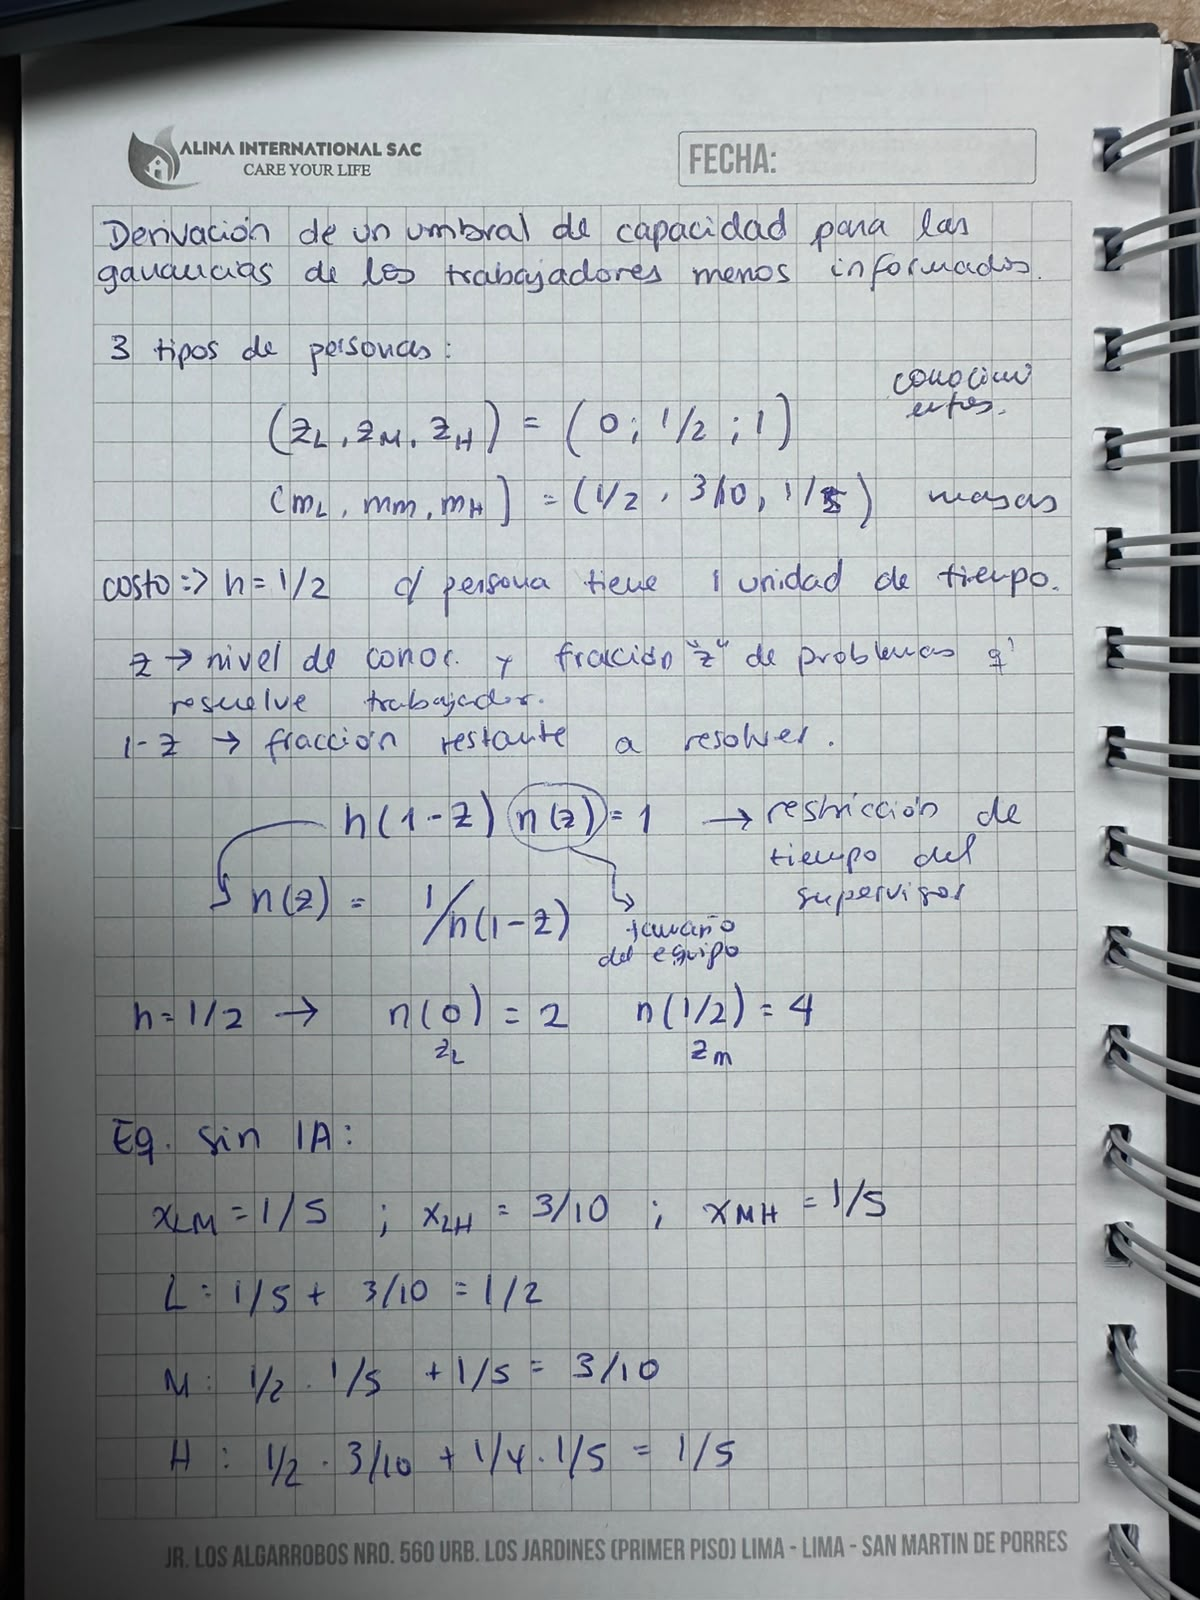
\includegraphics[height=.78\textheight,width=\linewidth,keepaspectratio]{hand/derivacion-01.jpeg}
\column{.49\textwidth}\centering
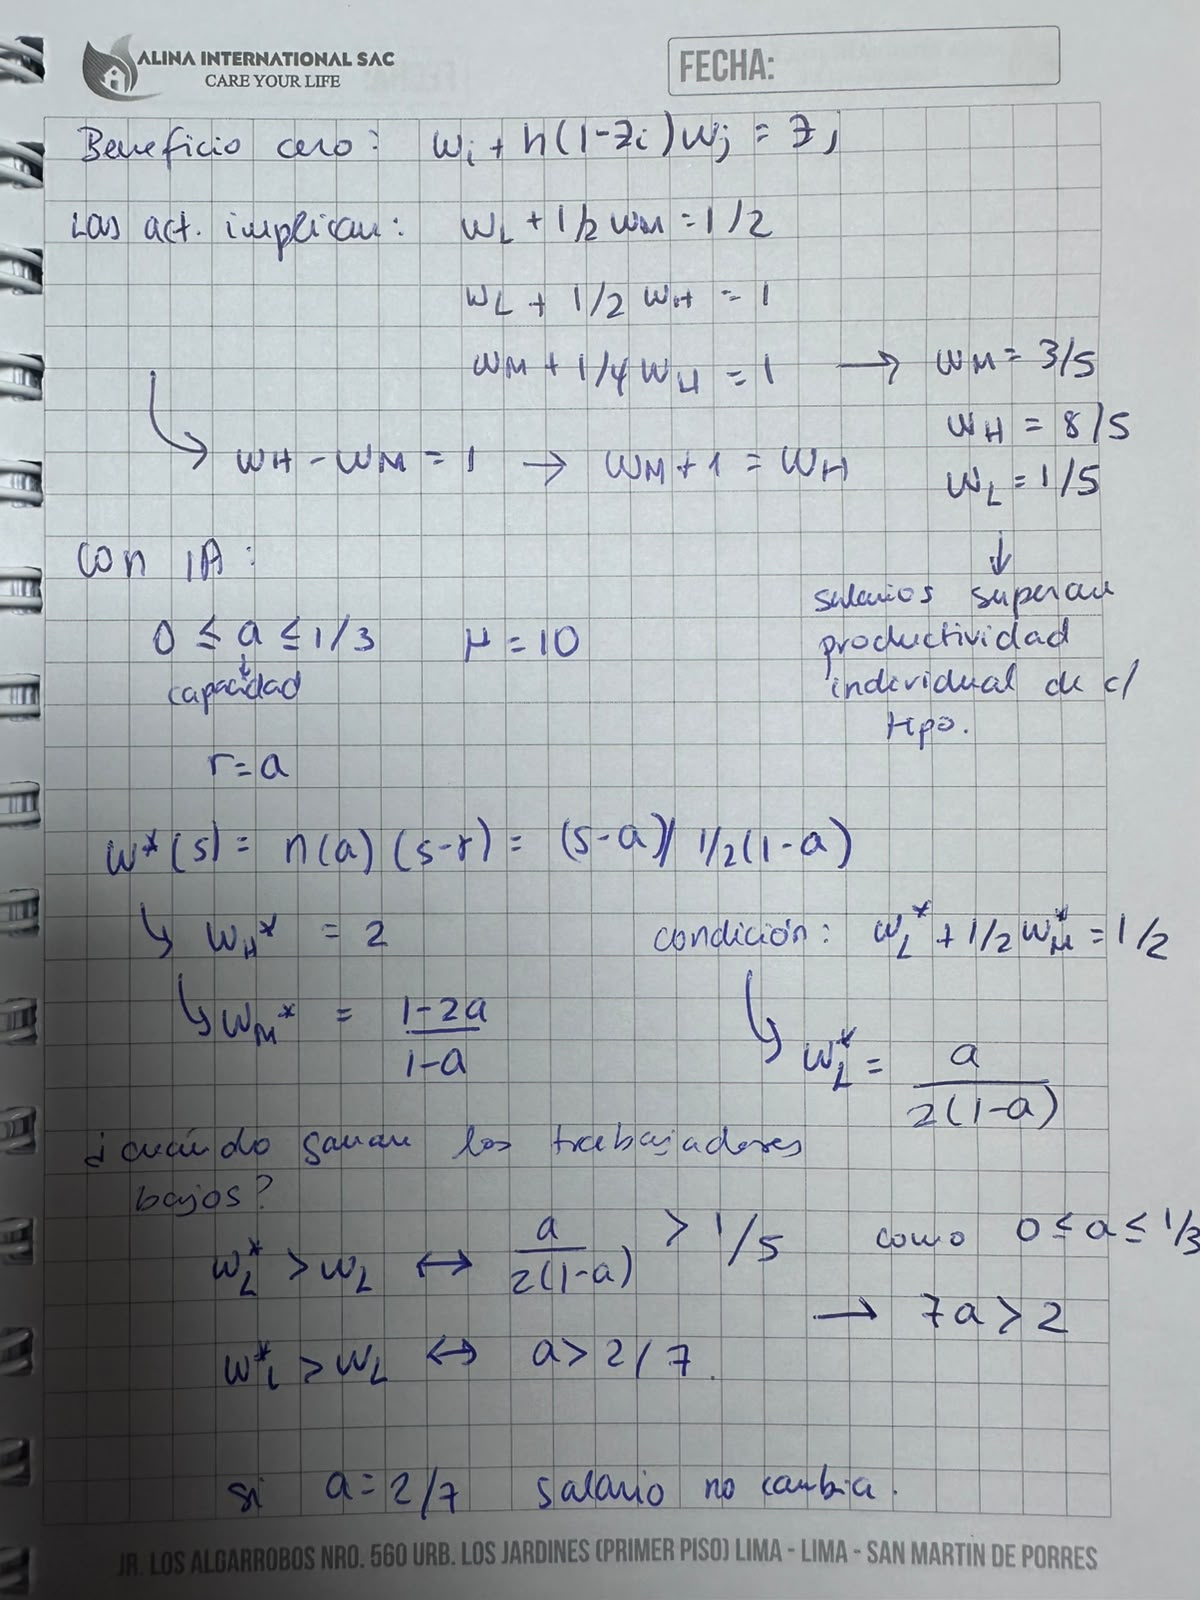
\includegraphics[height=.78\textheight,width=\linewidth,keepaspectratio]{hand/derivacion-02.jpeg}
\end{columns}
\vfill\centering\scriptsize Original photographs supplied by the student. Handwriting preserved in Spanish.
\end{frame}
\begin{frame}{Extension: output can rise while labor income falls}
\small
In our autonomous three-type economy, for $0\le a\le1/3$:
\[
\mathcal L^*(a)=\tfrac12\wa_L+\tfrac3{10}\wa_M+\tfrac15\wa_H
=\frac{14-15a}{20(1-a)}.
\]
\[
\frac{d\mathcal L^*}{da}=-\frac{1}{20(1-a)^2}<0,
\qquad
\frac{dY^*}{da}=\mu-\frac{1}{20(1-a)^2}>0\quad(\mu=10).
\]
Low wages rise and high wages stay fixed. Falling middle wages dominate the change in aggregate labor income.

This compares \emph{different autonomous capabilities}. Labor income still exceeds the no-AI baseline throughout this interval.
\vfill\footnotesize Own extension; exact symbolic verification. No claim is made outside this interval.
\end{frame}
\begin{frame}{Source version and reproducibility}
\small
Ide, E., \& Talam\`as, E. (2025). \emph{Artificial Intelligence in the Knowledge Economy}. JPE 133(12), 3762--3800.\par
\href{https://doi.org/10.1086/737233}{doi:10.1086/737233}

Read and pinned: \href{https://arxiv.org/abs/2312.05481v11}{arXiv:2312.05481v11}, 35 pages, title page February 25, 2025. The deposit metadata says February 24. The course's May manuscript and arXiv v12 were not substituted.

\texttt{analysis/}: derivation and solver.\quad\texttt{results/}: checks and data.\par
\texttt{lean/}: complete generated paper folder, preserving workflow artifacts.\par
\texttt{LEAN\_RUN.md}: exact run, scope, build/check result and blockers.

\href{https://github.com/davidolano03/ai-05-ide}{github.com/davidolano03/ai-05-ide}
\end{frame}
\end{document}
